%%%%%%%% ttwo women reverse
%% We start with a full minipage enclosing everything with it. This enables scaling of the
%% contents at a later stage
% This was one of the better templates that I used for the tex.stackexchange.com
% competition. Based on minipages and a bit of pulling and pushing. If you want to
% get fussy, some improvements in kerning are necessary. The left
% bottom caption was pushed using a rule. Set the rule height to 1pt to see
% how it was done.
% This has the rows reveresed than te twowomen template
% Dr Y Lazarides 2012
% 
\documentclass[imperial]{octavo}
\usepackage[top=1cm,left=0.5cm,right=0.5cm]{geometry}
\usepackage{graphicx}
\usepackage{caption}
\usepackage{multicol}
\usepackage{ragged2e}
\long\def\note{%
   \begin{minipage}[b]{2cm}
   \RaggedRight
   University of Pensylvania medical students for \$750. But Thomas Eskins became
                                   so interested that he painted an entire cancer operation,
                                    with portraits of student spectators thrown in.
  \end{minipage}
}
\parindent0pt
\begin{document}
\begin{minipage}{0.9\textwidth}
\vspace{\baselineskip}
\parindent0pt
\fboxrule0pt
{
\centering
\fbox{\centering
\begin{minipage}[t]{0.89\textwidth}
\centering
\begin{minipage}[t]{0.41\textwidth}
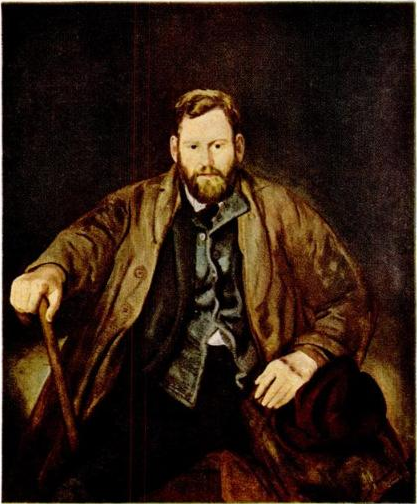
\includegraphics[width=1\textwidth]{threewomen01}\vspace*{-8pt}%
\captionof*{figure}{\noindent\footnotesize\textbf{WALDO PEIRCE}, a famous painting in his own right,
turned model for Bellows, posed for this impressive portrait in New York studio in 1920.}
\end{minipage}\hspace{0.5cm}
\begin{minipage}[t]{0.4\textwidth}
   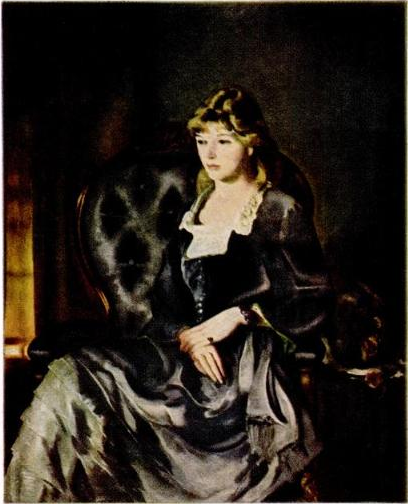
\includegraphics[width=1\textwidth]{threewomen02}\vspace*{-8pt}
    \captionof*{figure}{\noindent\footnotesize\textbf{MRS KATHERINE ROSEN,}
                 the daughter of Charles Rosen, he was an artist and neighbor of bellows, 
                 posed for this  meditative study in 1921.}
\end{minipage}
\end{minipage}
}}
%% This is the bottom picture
\medskip

\fbox{\hskip-0.3cm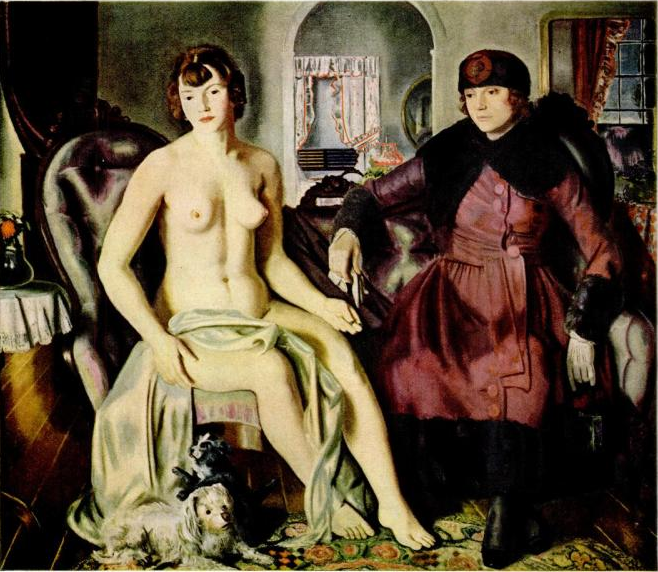
\includegraphics[width=\textwidth]{twowomen-03}}\\[-27.5pt]
\setlength{\linewidth}{0.95\textwidth}
\setlength{\columnsep}{8pt}
\begin{multicols}{2}
\noindent \footnotesize\textbf{TWO WOMEN,} portrays a professional model dressed and undressed. The range and richness of colors is unusual among Bellows' pictures. Bellows always had a horror of studio pictures and ``pretty nudes,'' rarely worked from professional models and never painted a still life.
\end{multicols}
\end{minipage}
\clearpage
\end{document}